\documentclass[tikz, border=10pt]{standalone}
\usepackage{xcolor}

% Define a custom green color for the tree nodes
\definecolor{treegreen}{HTML}{2E7D32}

\begin{document}
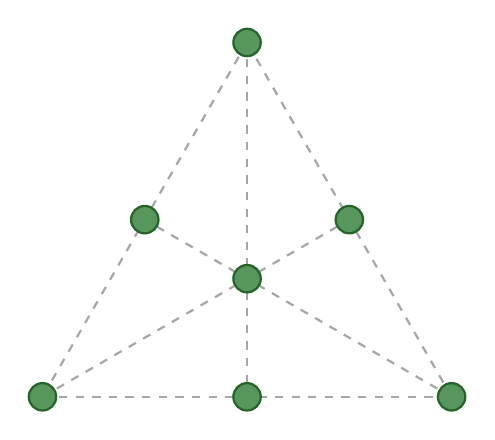
\begin{tikzpicture}[
    % Custom style for tree nodes
    tree/.style={
        circle, 
        draw=treegreen!80!black, 
        fill=treegreen!80, 
        inner sep=3.5pt, 
        thick
    },
    % Custom style for the row lines
    row line/.style={
        thick, 
        gray!70, 
        dashed
    }
]

  % 1. DEFINE COORDINATES using Polar Coordinates (angle:radius)
  
  % Centroid
  \coordinate (Center) at (0,0);
  
  % Outer Vertices (300°, 60°, 180° offset by 120° each)
  \coordinate (A) at (90:3cm);   % Top Vertex
  \coordinate (B) at (210:3cm);  % Bottom-Left Vertex
  \coordinate (C) at (330:3cm);  % Bottom-Right Vertex
  
  % Midpoints of the sides (halfway distance = 1.5cm)
  \coordinate (M_AB) at (150:1.5cm); % Left Midpoint
  \coordinate (M_BC) at (270:1.5cm); % Bottom Midpoint
  \coordinate (M_CA) at (30:1.5cm);  % Right Midpoint

  % 2. DRAW THE 6 ROWS OF 3 TREES EACH
  
  % Outer Triangle Sides (3 rows)
  \draw[row line] (A) -- (B);
  \draw[row line] (B) -- (C);
  \draw[row line] (C) -- (A);
  
  % Medians passing through the center (3 rows)
  \draw[row line] (A) -- (M_BC);
  \draw[row line] (B) -- (M_CA);
  \draw[row line] (C) -- (M_AB);

  % 3. DRAW THE 7 TREES (NODES)
  \node[tree] at (A) {};
  \node[tree] at (B) {};
  \node[tree] at (C) {};
  \node[tree] at (M_AB) {};
  \node[tree] at (M_BC) {};
  \node[tree] at (M_CA) {};
  \node[tree] at (Center) {};

\end{tikzpicture}
\end{document}
